\documentclass[12pt, a4paper]{article}
\usepackage{amsmath}
\usepackage{amsfonts}
\usepackage{amsthm}
\usepackage{mathtools}
\newtheorem{theorem}{Theorem}
\usepackage{pgfplots}
\pgfplotsset{width=10cm,compat=1.9}

\title{The gamma distribution}
\author{Kristian Wichmann}

\begin{document}

\maketitle

The graph below shows a few of the possible shapes:

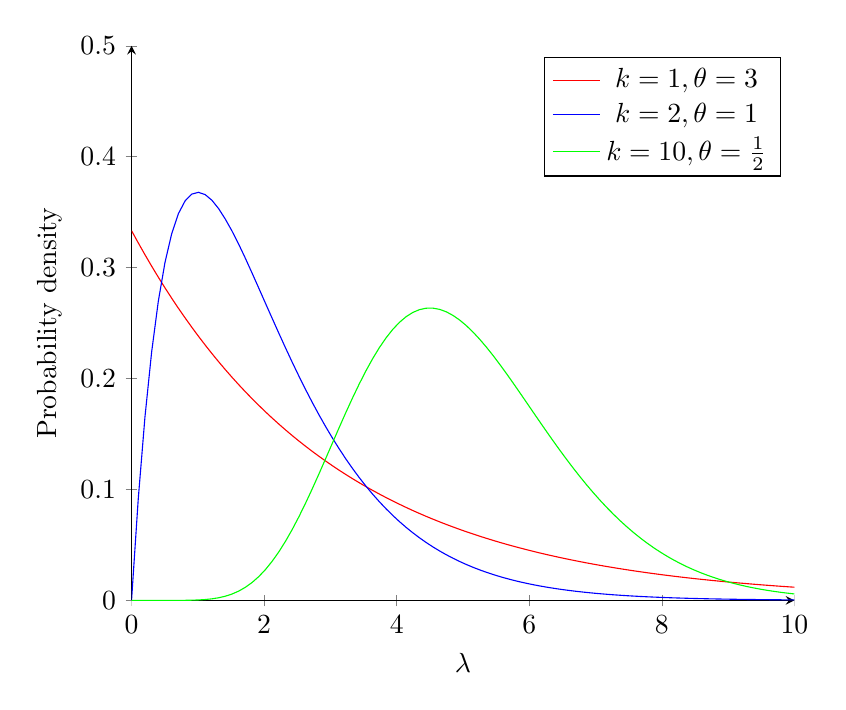
\begin{tikzpicture}
\begin{axis}[
    axis lines = left,
    xlabel = $\lambda$,
    ylabel = Probability density,
    ymin = 0,
    ymax = 0.5,
]
\addplot [
    domain=0:10, 
    samples=100, 
    color=red,
	]
	{pow(2.71828,-x / 3) / 3};
\addlegendentry{$k=1,\theta=3$}
\addplot [
    domain=0:10, 
    samples=100, 
    color=blue,
    ]
    {x * pow(2.71828,-x)};
\addlegendentry{$k=2,\theta=1$}
\addplot [
    domain=0:10, 
    samples=100, 
    color=green,
    ]
    {2^10 * x^9 * pow(2.71828,-x * 2) / 362880};
\addlegendentry{$k=10,\theta=\frac{1}{2}$}
 
\end{axis}
\end{tikzpicture}

\end{document}